\documentclass{article}

\usepackage[utf8]{inputenc} % Use UTF-8 encoding
\usepackage{textgreek} % For Greek letters

\usepackage{algorithm}
\usepackage{algpseudocode}
\usepackage{hyperref}
\usepackage{fourier}
\usepackage{tikz}
\usepackage{array}

\DeclareMathAlphabet{\mathcal}{OMS}{cmsy}{m}{n}
\SetMathAlphabet{\mathcal}{bold}{OMS}{cmsy}{b}{n}
\newcommand{\bigO}{\mathcal{O}}

\begin{document}

\section{Introduction}
Sorting algorithms on modern computers have been playing an important role in Computer Science and can date back to the early 50s and 60s. 
It is the great efforts that humans have put into the field of developing faster sorting algorithms that shapes the vital parts that formed
all the significant infrastructures of the vast computer world like databases, data centers, cluster networks etc.
In the realm of sorting algorithms, Quicksort, introduced by computer scientist Tony Hoare \cite{HoareQuickSort} to the public,
has made its way into the libc of the GNU/Linux system and stood the test of time as one of the most classical and widely used methods for sorting. 
Its divide-and-conquer strategy has been widely used and taken into research to fully utilize the performance of sorting.
The basic Quicksort picks an arbitrary pivot element,
partitions the array into 2 segments, one with elements less than the pivot and the other greater. 
It then recursively sorts these segments using the same method. While the original Quicksort method has proven effective,
the quest of further optimizations and the endless pursuit of efficiency has led to many variations to explore, one of which is the Multi-Pivot Quicksort. 

This thesis is my shallow attempt to unveil the benefits of Multi-Pivot Quicksort, exploring the effects more pivots can bring,
followed by some potential implementations and the analysis on the benefits that arise from leveraging multiple pivots in the Quicksort process.

\subsection{History and Related work}

When Quicksort was first invented a great number of variations and modifications were put into research over the years, 
such as sorting with a better partition method and a more optimal strategy to select the arbitrary pivot element.
But the innovative approach of Multi-pivot Quicksort, exemplified by Vladimir Yaroslavskiy \cite{Yaroslavskiy} in 2009,
Bentley and Bloch's algorithm (YBB Alogorithm), which was also highlighted by Wild and Nebel, adopted in Sun's Java 7 runtime library, 
introduces the use of two pivots. Contrary to initial expectations, studies have revealed that employing multiple pivots can enhance the performance,
challenging prior assumptions derived from the dual-pivot proposal by Sedgewick \cite{Sedgewick} in 1978 where he analyzed a potential dual-pivot approach, 
which was deemed inferior to the classical Quicksort in his research. Furthermore, Kushagra presented a 3-pivot Quicksort \cite{Kushagra} algorithm at ALENEX,
has attracted significant attention, further pushing the researches of multi-pivot strategies. 

One common pitfall in the performance downgrade of the conventional Quicksort is the degenerated cases,
which could often arise when the input array is already mostly sorted or when certain patterns in the data cause the algorithm to consistently choose poor pivots
that fail to split the data into evenly sized partitions. 
In such cases, the partitioning process may result in highly imbalanced partitions where the size of one partition is significantly larger than the other, leading to suboptimal performance and
potentially degrading the time complexity to $\bigO(n^2)$ instead of the expected $\bigO(n\log n)$ for Quicksort.
Wiser choices of pivot selections could decrease the possiblities of such events from happening, such as the median-of-3 method and its variations of median-of-5 and median-of-7.
But on mostly ascending or descending arrays, the median-of-3 method still has a chance of choosing the smallest or largest element as the pivot,
which is not the best ideal approach to prevent the worst case from happening. It also brings to our concerns that in real world applications, duplicated elements are not rare,
and the median-of-3 method could be easily affected by the duplicated elements, which could lead to the same worst case as the original Quicksort. 
There are some other variations of Quicksort that have been proposed to address these specific issues, such as the Introsort algorithm \cite{Introsort} by David Musser,
which switches to Heapsort when the recursion depth exceeds a certain threshold. Thus the worst running time is guaranteed to be $\bigO(n\log n)$ by doing so.

And this is where Multi-pivot quicksort comes into play. Assuming we are dealing with randomly generated arrays,
since we don't know the exact size of each partition, the more pivots we choose, the more partitions we divide the array into,
the less chance it will be that we encounter imbalanced sizes of partitions. 
Moreover, choosing more pivots will significantly reduce the chance we access the same elements again and the maximum depth of recursion,
which can translate into better running time. With n pivots we are dividing the array into n+1 partitions, the same things happen on the sub-partitions 
in the next level of recursion and we can conclude the maximum depth of recursion would be $\log_{n+1} L$ given \textbf{n} as the number of pivots and \textbf{L} for the length of array.
Greater the n is, less the depth. Better memory behaviors can bring effects that can not be achieved by any of other traditional means such as choosing a better pivot value
among samples extracted from different parts of the array, but the drawbacks are also obvious, 
branch misprediction could be terrible as the different outcomes of comparisons can largely impact on the runtime performance.
A delay of 14 to 19 stages on a typical Intel desktop CPU or 20 to 25 stages on AMD's Zen CPUs could lead to huge efficiency loss for our algorithm,
and this number only grows as the number of pivots increases and on more complicatad architectures. These are the trade-offs we have to consider when we are choosing the number of pivots,
although these side effects can be mitigated by the use of branchless comparisons and modern CPUs are able to run conditional move operations (cmove) to avoid branches,
these overheads still remain as concerns.
Apart from that, it could be really tricky when it comes to moving the elements to the right places among multiple partitions, especially when the number of pivots is large.
Additionally, comparisons are the second expensive things next to swaps we are dealing with, and the more pivots we choose, the more comparisons we have to make.
Even for the case of using only one pivot, the average number of comparisons remain unoptimial, being $1.38n\log n + \bigO(n)$ compared with the $n\log n + \bigO(n)$ of the Merge Sort,
but the overall instructions are much less than the average of Merge Sort and with proper pivot selection strategy, it can still be reduced to a certain extent.

% As the number of pivots increase, it is important that we take the worst cases into consideration. 
% Will we end up wasting too much time on comparing with badly-chosen similar pivots that split the array into imbalanced partitions,
% one of which might have much larger size than the rest? Or Even with the relatively higher amount of branch mispredictions, 
% will we still conquer the barriers of cache misses caused by long-lasting swaps of elements far away and reach a shorter time as the n grows?
% That's the riddle I'm going to research in the next section.

Fortunately, an efficient approach has been put forward by Stefan Edelkamp and Armin Weiß,
in their thesis of BlockQuickSort \cite{BlockQuickSort}
which evens the odds of both branch mis-prediction and cache misses which uses one or more buffer blocks of constant sizes on the stack
to store the index offsets of out-of-order elements, swap them altogether in a second pass to rearrange them in order
after scanning a large chunk of array with the size of the block. Their approach realized a significant speedup up to 80\% faster compared with the GCC implementation of std sort
with only one single pivot. The BlockQuickSort has been adapted to the Multi-Pivot Quicksort and the results are also promising,
the improvements on contiguous memory access significantly improves the spatial locality and reduces both the cache misses and branch mis-predictions.
Branchless comparisons are also adapted which plays an important role in contributing to the huge performance boost by reducing the overhead
when increasing the counter of elements stored in the block buffer(s).
This novel approach has also developed variations that could effectively make the use of different partitioning methods and multiple pivots selected. 

Meanwhile, in the pursuit of advancing the efficiency of the Quicksort algorithm,
my investigation led me to explore various modifications, 
with a particular focus on the pattern-defeating Quicksort (PDQSort) proposed by Orson Peters. 
PDQSort leverages the average-case performance of randomized Quicksort with the rapid worst-case execution of heapsort, 
while concurrently achieving linear time complexity for slices exhibiting specific patterns. 
Notably, PDQSort employs a judicious application of randomization to prevent the degenerated case from happening.
When it does, PDQSort will strategically shuffle or reverse the entire array to simplify the sorting and increase the speed.
If all the counter measures fail, it also has the final backup plan of switching to Heapsort when bad choices of pivots or the depth of recursions exceed the limit. 
In terms of pivot selection, it uses a fixed seed when generating a pseudo-random index to ensure the reproducibility and deterministic behavior.
Furthermore, in instances where randomly selected elements from the original array appear in a descending order.
The combination of these optimizations has demonstrated a significant enhancement in performance, showcasing PDQSort as up to twice faster than the original Quicksort algorithm. 
This outcome illuminates the transformative impact that a comprehensive analysis on the pattern of arrays has on the speed of sorting algorithms,
not to mention it is a successful combination of BlockQuickSort's partition method,
Heap sort when dealing with worst cases and Insertion sort when it comes to small sub-arrays of sizes less than the cache line size. 
Inspired by PDQSort's success, I dive into the diverse variations of Quicksort,
motivating a search for novel patterns that may be leveraged to enhance the existing Quicksort algorithms.

\subsection{Contributions}
\begin{itemize}
    \item Present the variants of Multi-Pivot QuickSort and implement a 4-Pivots Quicksort and evaluate N-Pivots Quicksort from N = 1, 2, 3, 4 experimentally. 
        Comparing the implementations, times, instructions, cache misses and branch mis-predictions with a duration of 3 seconds warm-up time.
    \item Present a new layout of Multi-Pivot BlockQuickSort that could potentially reduce the memory access and increase the block buffer usage rate. 
        Analyze this method with all other available variants with block partitioning and compare the pros and cons.
\end{itemize}

\section{Preliminaries}
\begin{algorithm}[H]
    \caption{QuickSort with Hoare Partition}\label{HoarePartition}
    \begin{algorithmic}[1]
        \Procedure{QuickSort}{$A, l, r$}
        \If{$l < r$}
        \State $p \gets \textsc{HoarePartition}(A, l, r)$
        \State \textsc{QuickSort}(A, l, p-1)
        \State \textsc{QuickSort}(A, p+1, r)
        \EndIf
        \EndProcedure
        \Procedure{HoarePartition}{$A, l, r$}
        \State $P \gets A[l]$ \Comment{Pivot}
        \State $i \gets l - 1$
        \State $j \gets r + 1$
        \While{$i < j$}
        \Repeat
        \State $j \gets j - 1$
        \Until{$A[j] < P$}
        \Repeat
        \State $i \gets i + 1$
        \Until{$A[i] > P$}
        \State \textsc{Swap}($A[i], A[j]$)
        \EndWhile
        \State \textsc{Swap}($A[l], A[j]$) \Comment{Put pivot in the middle}
        \State \textbf{return} $j$
        \EndProcedure
    \end{algorithmic}
\end{algorithm}

For Quicksorts with single pivot value, the partitioning procedure splits the array into 2 parts where the left part are elements less than the pivot and the right part being greater, 
separated by the pivot value in the middle. Then the main body recursively sorts the left and right part to rearrange all the elements in the correct order. The hoare's partition method
uses double pointers starting at the leftmost and the rightmost element in the array and scanning towards the middle until they meet. Each pointer scans for mis-placed elements 
which belong to the other partition by comparing the current element to the pivot. 
Out-of-order elements are swapped in pairs to the right place and the scanning procedure continues until all elements 
are moved to the places where they belong.

\begin{algorithm}[H]
    \caption{QuickSort with Lomuto Partition}\label{LomutoPartition}
    \begin{algorithmic}[1]
        \Procedure{QuickSort}{$A, l, r$}
        \If{$l < r$}
        \State $p \gets \textsc{LomutoPartition}(A, l, r)$
        \State \textsc{QuickSort}(A, l, p-1)
        \State \textsc{QuickSort}(A, p+1, r)
        \EndIf
        \EndProcedure
        \Procedure{LomutoPartition}{$A, l, r$}
        \State $P \gets A[r]$ \Comment{Pivot}
        \State $i \gets l$
        \For{$j \gets l$ \textbf{to} $r-1$}
        \If{$A[j] < P$}
        \State \textsc{Swap}($A[i], A[j]$)
        \State $i \gets i + 1$
        \EndIf
        \EndFor
        \State \textsc{Swap}($A[i], A[r]$) \Comment{Put pivot in the middle}
        \State \textbf{return} $i$
        \EndProcedure
    \end{algorithmic}
\end{algorithm}

While the Lomuto partition method uses another way, it scans the array in sequential order from left to right using one bare pointer, ascending the index by 1 each time.
and swaps all the elements less than the pivot to the left side regardless,
thus duplicated swaps are introduced due to not checking if the elements are already in the right places. Both of these 2 partition methods are straightforward, 
and their main structures are similar: scan, find mis-placed elements, swap and recursively repeat the same procedure until the whole array is sorted.

\begin{algorithm}[H]
    \caption{Dual-Pivot QuickSort}\label{DualPivotQuickSort}
    \begin{algorithmic}[1]
        % \Procedure{DualPivotQuickSort}{$A, l, r$}
        % \If{$l < r$}
        % \State $p1, p2 \gets \textsc{DualPivotPartition}(A, l, r)$
        % \State \textsc{DualPivotQuickSort}(A, l, p1-1)
        % \State \textsc{DualPivotQuickSort}(A, p1+1, p2-1)
        % \State \textsc{DualPivotQuickSort}(A, p2+1, r)
        % \EndIf
        % \EndProcedure

        \Procedure{DualPivotPartition}{$A, l, r$}
        \State $P1, P2 \gets A[l], A[r]$ \Comment{Pivots}
        \If{$P1 > P2$}
        \State \textsc{Swap}($P1, P2$)
        \EndIf

        \State $less \gets l + 1$
        \State $greater \gets r - 1$

        \State $k \gets l$
        \While{$k \leq greater$}
            \If{$A[k] < P1$} \Comment{If the current element is less than P1}
                \State \textsc{Swap}($A[k], A[less]$) \Comment{Shift the element to the leftmost partition}
                \State $less \gets less + 1$
            \ElsIf{$A[k] > P2$} \Comment{If the current element is greater than P2}
                \While{$A[greater] > P2$ \textbf{and} $k < greater$}
                    \State $greater \gets greater - 1$ \Comment{Find the first element less than P2}
                \EndWhile
                \State \textsc{swap}(A[k], A[greater]) \Comment{Swap to the rightmost partition}
                \State $greater \gets greater - 1$
    
                \If{$A[j] < P1$} \Comment{Double check if another swap is needed}
                    \State \textsc{Swap}($A[k], A[less]$) 
                    \State $less \gets less + 1$
                \EndIf
            \EndIf
            \State $k \gets k + 1$ \Comment{Move to the next element}
        \EndWhile
        \State $less \gets less - 1$
        \State $greater \gets greater + 1$
        \State \textsc{Swap}($A[l], A[less]$) \Comment{Put Pivot1 in the middle}
        \State \textsc{Swap}($A[r], A[greater]$) \Comment{Put Pivot2 in the middle}
        \State \textbf{return} $less, greater$
        \EndProcedure
    \end{algorithmic}
\end{algorithm}

With one more pivot added, the two-pivot Quicksort method is introduced by Vladimir Yaroslavskiy in 2009. It uses 2 pivots selected from each end to split the array into 3 parts.
K stands for the current element being scanned, it will be swapped to the left part, which is accumulated by the less pointer, if it is less than the first pivot or do nothing if it is in the middle part.
Otherwise, if it is greater than the second pivot, it will be swapped to the right part, which is accumulated by the greater pointer.
We will double check the current element at index k after the swap to see if it is less than the first pivot, if so, we will swap it to the left part and move the less pointer to the right.
Hereby, we can see that the Dual-Pivot Quicksort is a generalization of the original Quicksort, and the partitioning method is also a generalization of the original Hoare's partition method but with 2 pivots.

What's attracting is that there was once a debate on whether multiple pivots could enhance the performance, as Sedgewick,
who analyzed a dual-pivot approach with an average of $\frac{32}{15}n \ln n + \bigO{n}$ comparisons in 1978, in constrast to the $2n\ln n + \bigO{n}$ of the standard Quick Sort, considered this prototype to be inferior to the classical Quicksort.
However, the Yaroslavskiy's Dual-Pivot Quicksort has proven to be a success, with the experimental results showing that it has a less amount of $1.9n\ln n + \bigO{n}$ amortized comparisons, but more swaps,
approximately $0.6n\ln n + \bigO{n}$ which is much greater than the $0.33n\ln n + \bigO{n}$ of the original one, is faster than the original Quicksort in most cases.
It is surprising that even with asymptotically only 5\% of less comparisons and nearly 80\% more swaps, the Dual-Pivot Quicksort still outperforms the original Quicksort in practice.
What makes this more mysterious, is the variation of Yaroslavskiy's partition method that always compares to the larger pivot, by Martin Aumüller and Martin Dietzfelbinger 2013 in their thesis of 'Optimal Partitioning for Dual Pivot Quicksort' \cite{OptimalPartitioningForDualPivotQuicksort}.
The method shows no difference in terms of both comparison and swaps with the original Dual-Pivot Quicksort, but it turned out that it is as fast as the Yaroslavskiy's partition, and even faster than another method along with it, named 'Countering Strategy C', who claimed to have the least 
estimations of $1.8n \ln n + \bigO(n)$ comparisons and $1.6n \ln n + \bigO{n}$ swaps. This is a great example of how the real-world performance could be different from the theoretical analysis. In fact, in their following tests, the 'Countering Strategy C' method was proven to be the slowest among all the 3 methods.

It is noteworthy the there still lies a huge gap between the theoretical analysis and the real-world performance. It is time we broaden our horizon and look for more factors that could contribute more to the change of the performance of the Quicksort algorithm.
The cache misses, branch mis-predictions, and the number of instructions are the things we should take into consideration when we are analyzing on mutated versions of the Quicksort algorithm.
Apparently, the number of pivots plays a significant role, and is one of the factors that could potentially bring a significant change. Let's dive deeper to see the world of 3-Pivots Quicksort.

\begin{algorithm}[H]
    \caption{3-Pivot QuickSort}\label{3PivotQuickSort}
    \begin{algorithmic}[1]
        \Procedure{ThreePivotPartition}{$A, l, r$}
        \State $P1, P2, P3 \gets A[l], A[l+1], A[r]$ \Comment{And sort 3 Pivots in ascending order} 

        \State $i, j \gets l + 2$
        \State $k, l \gets r - 1$
        \While{$j \leq k$}
            % // j moves right until arr[j] >= p2
            % while arr[j].cmp(&p2) == Ordering::Less {
            %     // arr[<i] -> elements that are less than p1, arr[i] is not less than p1
            %     if arr[j].cmp(&p1) == Ordering::Less {
            %         arr.swap_unchecked(i, j);
            %         i += 1;
            %     }
            %     j += 1;
            % }
            \While{$A[j] < P2$} \Comment{Put left side elements less than P2 in order}
                \If{$A[j] < P1$}
                    \State \textsc{Swap}($A[i], A[j]$)
                    \State $i \gets i + 1$
                \EndIf
                \State $j \gets j + 1$
            \EndWhile
            % // k moves left until arr[k] <= p2
            % while arr[k].cmp(&p2) == Ordering::Greater {
			% 	// arr[>l] -> elements that are greater than p3, arr[l] is not greater than p3
			% 	if arr[k].cmp(&p3) == Ordering::Greater {
			% 		arr.swap_unchecked(k, l);
			% 		l -= 1;
			% 	}
			% 	k -= 1;
			% }
            \While{$A[k] > P2$} \Comment{Put right side elements greater than P2 in order}
                \If{$A[k] > P3$}
                    \State \textsc{Swap}($A[k], A[l]$)
                    \State $l \gets l - 1$
                \EndIf
                \State $k \gets k - 1$
            \EndWhile
			% // if j is still less than k
			% if j <= k {
			% 	if arr[j].cmp(&p3) == Ordering::Greater {
			% 		if arr[k].cmp(&p1) == Ordering::Less {
			% 			// if arr[j] > p3 and arr[k] < p1, 
			% 			// rotate arr[j] to k and arr[k] to i because arr[<i] < p1
			% 			rotate3(arr, [j, i, k]);
			% 			i += 1;
			% 		} else {
			% 			// if arr[j] > p3 and arr[k] >= p1,
			% 			// simply swap arr[j] and arr[k]
			% 			arr.swap_unchecked(j, k);
			% 		}
			% 		// at this moment arr[k] must be greater than p3
			% 		// swap it with arr[l] to move it to the right
			% 		arr.swap_unchecked(k, l);
			% 		l -= 1;
			% 	} else { 
			% 		// if arr[j] <= p3, we do the same logic as above
			% 		if arr[k].cmp(&p1) == Ordering::Less {
			% 			rotate3(arr, [j, i, k]);
			% 			i += 1;
			% 		} else {
			% 			arr.swap_unchecked(j, k);
			% 		}
			% 		// at this moment arr[j] must be less than or equal p1
			% 		// arr[k] must be less than or equal p3
			% 	}
			% 	j += 1;
			% 	k -= 1;
			% }
            \If{$j \leq k$}
                \If{$A[j] > P3$} \Comment{Deal with 2 branches when A[j] is greater than P3}
                    \If{$A[k] < P1$}
                        \State \textsc{Rotate3}($A, [j, i, k]$)
                        \State $i \gets i + 1$
                    \Else
                        \State \textsc{Swap}($A[j], A[k]$) \Comment{A[j] > P3 and P2 > A[k] $\ge$ P1}
                    \EndIf
                    \State \textsc{Swap}($A[k], A[l]$)
                    \State $l \gets l - 1$
                \Else \Comment{Deal with 2 branches when A[j] is less than or equal to P3}
                    \If{$A[k] < P1$}
                        \State \textsc{Rotate3}($A, [j, i, k]$)
                        \State $i \gets i + 1$
                    \Else
                        \State \textsc{Swap}($A[j], A[k]$)
                    \EndIf
                \EndIf
                \State $j \gets j + 1, k \gets k - 1$
            \EndIf
        \EndWhile
        \State $i \gets i - 1, j \gets j - 1, k \gets k + 1, l \gets l + 1$
        % rotate3(arr, [left + 1, i, j]);
        \State \textsc{Rotate3}($A, [left + 1, i, j]$)
        % arr.swap_unchecked(left, i);
		% arr.swap_unchecked(right, l);
        \State \textsc{Swap}($A[left], A[i]$)
        \State \textsc{Swap}($A[right], A[l]$)
        \State \textbf{return} $i, j, l$
        \EndProcedure
    \end{algorithmic}
\end{algorithm}


The three-pivot Quicksort, introduced by Shrinu Kushagra, uses the similar hoare-like partition method, is a further generalization of the Dual-Pivot Quicksort.
In the original implementation, the 3 pivots are selected from the leftmost, the second element and the rightmost element of the array, and are sorted in ascending order.
The scanning procedure is similar to the Dual-Pivot Quicksort, but with 3 pivots, the array is divided into 4 parts, and is repeated until all elements are set.
The i, j, k, l pointers are used to scan the array and the elements are swapped to the right places according to the comparison results with the 3 pivots,
where i stands for the leftmost part where elements less than Pivot 1 belongs, j stands for the middle-left part, k stands for the middle-right part and l stands for the rightmost part.
Between j and k stands the unknown region where elements are not yet compared with any of the pivots. 
If the elementa at index j is less than Pivot 2, it is whether swapped to the leftmost part if it is less than Pivot 1,
or do nothing otherwise, since the middle-left part is for elements greater than Pivot1 and less than or equal to Pivot 2.
Same logic applies to the rightmost part, where elements are greater than Pivot 2 and less than or equal to Pivot 3.
These two pre-conditions are checked before the main body of the swapping and rotating procedure, which corresponds to the 2 while loops applied at the top of the main scanning loop.
Afterwards, the real swapping and rotating procedure is applied to the elements at index j and k, which are on the left and right boundaries of the unknown region, need to go to the other side of the array and moved to the right places.

We can simplify this part into a 2 if-else nested block, where the outter if-else block is for the case at index j and the inner one is for the case at index k (vice versa, but we will not go into details here).
Both of them have 2 branches, one for the case where the current element belongs to the leftmost or the rightmost part, and the other for the case where it belongs to the middle-left or the middle-right part.
It is not hard to tell there are $2 \times 2 = 4$ branches in total, and the swapping and rotating procedure is applied to each of them. The following chart \hyperlink{fig:3pivot}{`} illustrates the 4 branches and the corresponding actions.

% \listoffigures
\begin{figure}[H]
    \hypertarget{fig:3pivot}{}
    \caption{3-Pivot Quick Sort}
    \centering
    \hspace*{-0.25\textwidth}
    % \vspace*{+0.1\textheight}
    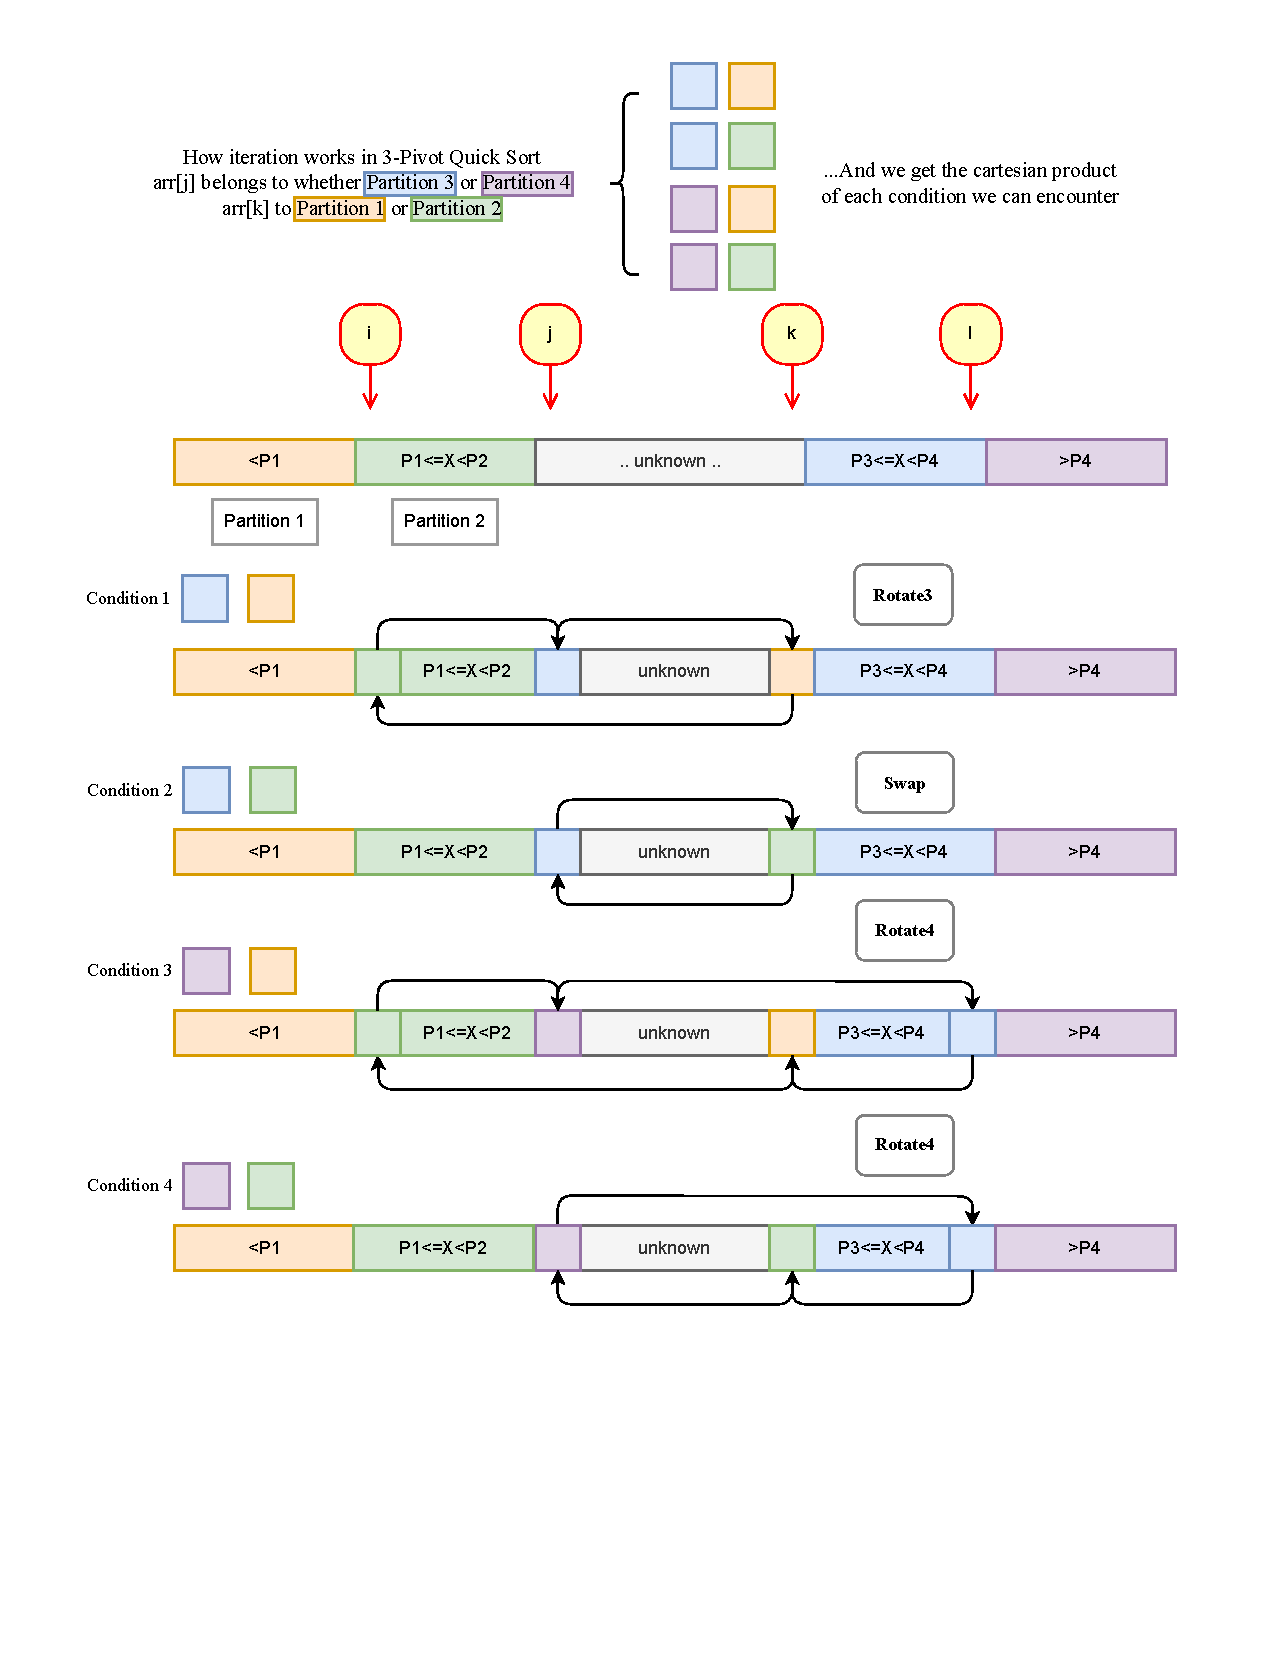
\includegraphics[width=1.5\textwidth]{3pivot.drawio.pdf}
\end{figure}

\begin{algorithm}[H]
    \caption{4-Pivot QuickSort}\label{4PivotQuickSort}
    \begin{algorithmic}[1]
        \Procedure{FourPivotPartition}{$A, l, r$}
        
        % let p1: *mut T = &mut arr[left];
		% let p2: *mut T = &mut arr[left + 1];
		% let p3: *mut T = &mut arr[right - 1];
        % let p4: *mut T = &mut arr[right];
        \State $P1, P2, P3, P4 \gets A[l], A[l+1], A[r-1], A[r]$ \Comment{And sort 4 Pivots in order} 

        % let (mut i, mut j, mut k, mut l, mut m) = (left + 2, left + 2, left + 2, right - 2, right - 2);
		% let (p1, p2, p3, p4) = (ptr::read(p1), ptr::read(p2), ptr::read(p3), ptr::read(p4));
        

        % while k <= l {
        %     //        | i              | j              | k
        %     // | < p1 | >= p1 and < p2 | >= p2 and < p3 | unknown
        %     while arr[k].cmp(&p3) == Ordering::Less {
        %         if arr[k].cmp(&p1) == Ordering::Less {
        %             rotate3(arr, [k, j, i]);
        %             i += 1;
        %             j += 1;
        %         } else if arr[k].cmp(&p2) == Ordering::Less {
        %             arr.swap_unchecked(k, j);
        %             j += 1;
        %         }
        %         k += 1;
        %     }
        \State $i, j, k, l, m \gets l + 2, l + 2, l + 2, r - 2, r - 2$
        \While{$k \leq l$}
            \While{$A[k] < P3$} \Comment{Put left side elements less than P3 in order}
                \If{$A[k] < P1$}
                    \State \textsc{Rotate3}($A, [k, j, i]$)
                    \State $i \gets i + 1$, $j \gets j + 1$
                \ElsIf{$A[k] < P2$}
                    \State \textsc{Swap}($A[k], A[j]$)
                    \State $j \gets j + 1$
                \EndIf
                \State $k \gets k + 1$
            \EndWhile
            % //        | l              | m              | 
            % // | >= p3 and < p4 | unknown
            % while arr[l].cmp(&p3) == Ordering::Greater {
            %     if arr[l].cmp(&p4) == Ordering::Greater {
            %         arr.swap_unchecked(l, m);
            %         m -= 1;
            %     }
            %     l -= 1;
            % }
            \While{$A[l] > P3$} \Comment{Put right side elements greater than P3 in order}
                \If{$A[l] > P4$}
                    \State \textsc{Swap}($A[l], A[m]$)
                    \State $m \gets m - 1$
                \EndIf
                \State $l \gets l - 1$
            \EndWhile
        %     if k <= l {
        %         if arr[k].cmp(&p4) == Ordering::Less {
        %             // arr[k] > p3, arr[l] < p3
        %             if arr[l].cmp(&p1) == Ordering::Less {
        %                 rotate4(arr, [k, j, i, l]);
        %                 i += 1;
        %                 j += 1;
        %             } else if arr[l].cmp(&p2) == Ordering::Less {
        %                 rotate3(arr, [k, j, l]);
        %                 j += 1;
        %             } else {
        %                 arr.swap_unchecked(k, l);
        %             }
        \If {$k \leq l$} \Comment{Start manipulation on the boundaries of unknown region}
            \If{$A[k] < P4$} \Comment{Deal with 3 branches when A[k] is less than P4}
                \If{$A[l] < P1$}
                    \State \textsc{Rotate4}($A, [k, j, i, l]$)
                    \State $i \gets i + 1$, $j \gets j + 1$
                \ElsIf{$A[l] < P2$}
                    \State \textsc{Rotate3}($A, [k, j, l]$)
                    \State $j \gets j + 1$
                \Else
                    \State \textsc{Swap}($A[k], A[l]$)
                \EndIf
        %         } else {
        %             // arr[k] > p4, arr[l] < p3
        %             if arr[l].cmp(&p2) == Ordering::Greater { // arr[l] goes to (p2, p3), increase k
        %                 rotate3(arr, [k, l, m]);
        %             } else if arr[l].cmp(&p1) == Ordering::Greater { // arr[l] goes to (p1, p2), increase j and k
        %                 rotate4(arr, [k, j, l, m]);
        %                 j += 1;
        %             } else { // arr[l] goes to leftmost side
        %                 rotate5(arr, [k, j, i, l, m]);
        %                 i += 1;
        %                 j += 1;
        %             }
        %             m -= 1;
        %         }
        %         k += 1;
        %         l -= 1;
        %     }
        % }
            \Else \Comment{Deal with 3 branches when A[k] is greater than P4}
                \If{$A[l] > P2$}
                    \State \textsc{Rotate3}($A, [k, l, m]$)
                \ElsIf{$A[l] > P1$}
                    \State \textsc{Rotate4}($A, [k, j, l, m]$)
                    \State $j \gets j + 1$
                \Else
                    \State \textsc{Rotate5}($A, [k, j, i, l, m]$)
                    \State $i \gets i + 1$, $j \gets j + 1$
                \EndIf
                \State $m \gets m - 1$
            \EndIf
            \State $k \gets k + 1$, $l \gets l - 1$
        \EndIf
        \algstore{4pivots}
    \end{algorithmic}
\end{algorithm}

\clearpage

\begin{algorithm}[H]
    \caption{4-Pivot QuickSort (Continued)}\label{4PivotQuickSort2}
    \begin{algorithmic}[1]
        \algrestore{4pivots}
        \EndWhile
        % i -= 1;
        % j -= 1;
        % // k -= 1;
        % l += 1;
        % m += 1;
        \State $i \gets i - 1, j \gets j - 1, k \gets k - 1, l \gets l + 1, m \gets m + 1$
        % // i, j, l, m are indexes of pivot 1, 2, 3, 4
        % // Here is the place rotate3 can't be replaced by arr.rotate_left
        % // because the indexes (left + 1 > i ?) are not always ascending
        % // so it could lead to a panic
        % // anyway, I leave the rotate_n macro for you to try out in `src/util.rs`
        % rotate3(arr, [left + 1, i, j]);
        % i -= 1;
        % arr.swap_unchecked(left, i);
        
        % rotate3(arr, [right - 1, m, l]);
        % m += 1;
        % arr.swap_unchecked(right, m);
        \State \textsc{Rotate3}($A, [left + 1, i, j]$)
        \State $i \gets i - 1$
        \State \textsc{Swap}($A[left], A[i]$)
        \State \textsc{Rotate3}($A, [right - 1, m, l]$)
        \State $m \gets m + 1$
        \State \textsc{Swap}($A[right], A[m]$)
        \EndProcedure
    \end{algorithmic}
\end{algorithm}

As long as the number of pivots increases, the number of branches will grow linearly, and the complexity of the partitioning method will also increase.
Thankfully, for 4-Pivot QuickSort \hyperlink{fig:4pivot}{`}, \hypertarget{2MoreBranches}we are just adding two more branches (As showed in the blue-red and purple-red branches in the chart below)
compared with the $2 \times 2 = 4$ branches for 3-Pivots into considerations and the branching logic is still under control.
We declare this as the balanced partition\hypertarget{BalancedPartition} layout we are using, where each side of the array is filled with $\frac{N + 1}{2}$ partitions for odd number $N$ of pivots, or one side with $\frac{N}{2}$ partitions and $\frac{N}{2} + 1$ on the other, we are going to have 9 branches for 5-Pivot QuickSort (3 partitions on each side, $3 \times 3 = 9$) and 12 branches for 6-Pivot QuickSort (3 partitions on one side and 4 on the other, $3 \times 4 = 12$).
The complexity of the partitioning method is growing way too far and thus only 4-Pivot QuickSort will be discussed in this thesis.

\begin{figure}[H]
    \hypertarget{fig:4pivot}{}
    \caption{4-Pivot Quick Sort}
    \centering
    \hspace*{-0.25\textwidth}
    % \vspace*{+0.1\textheight}
    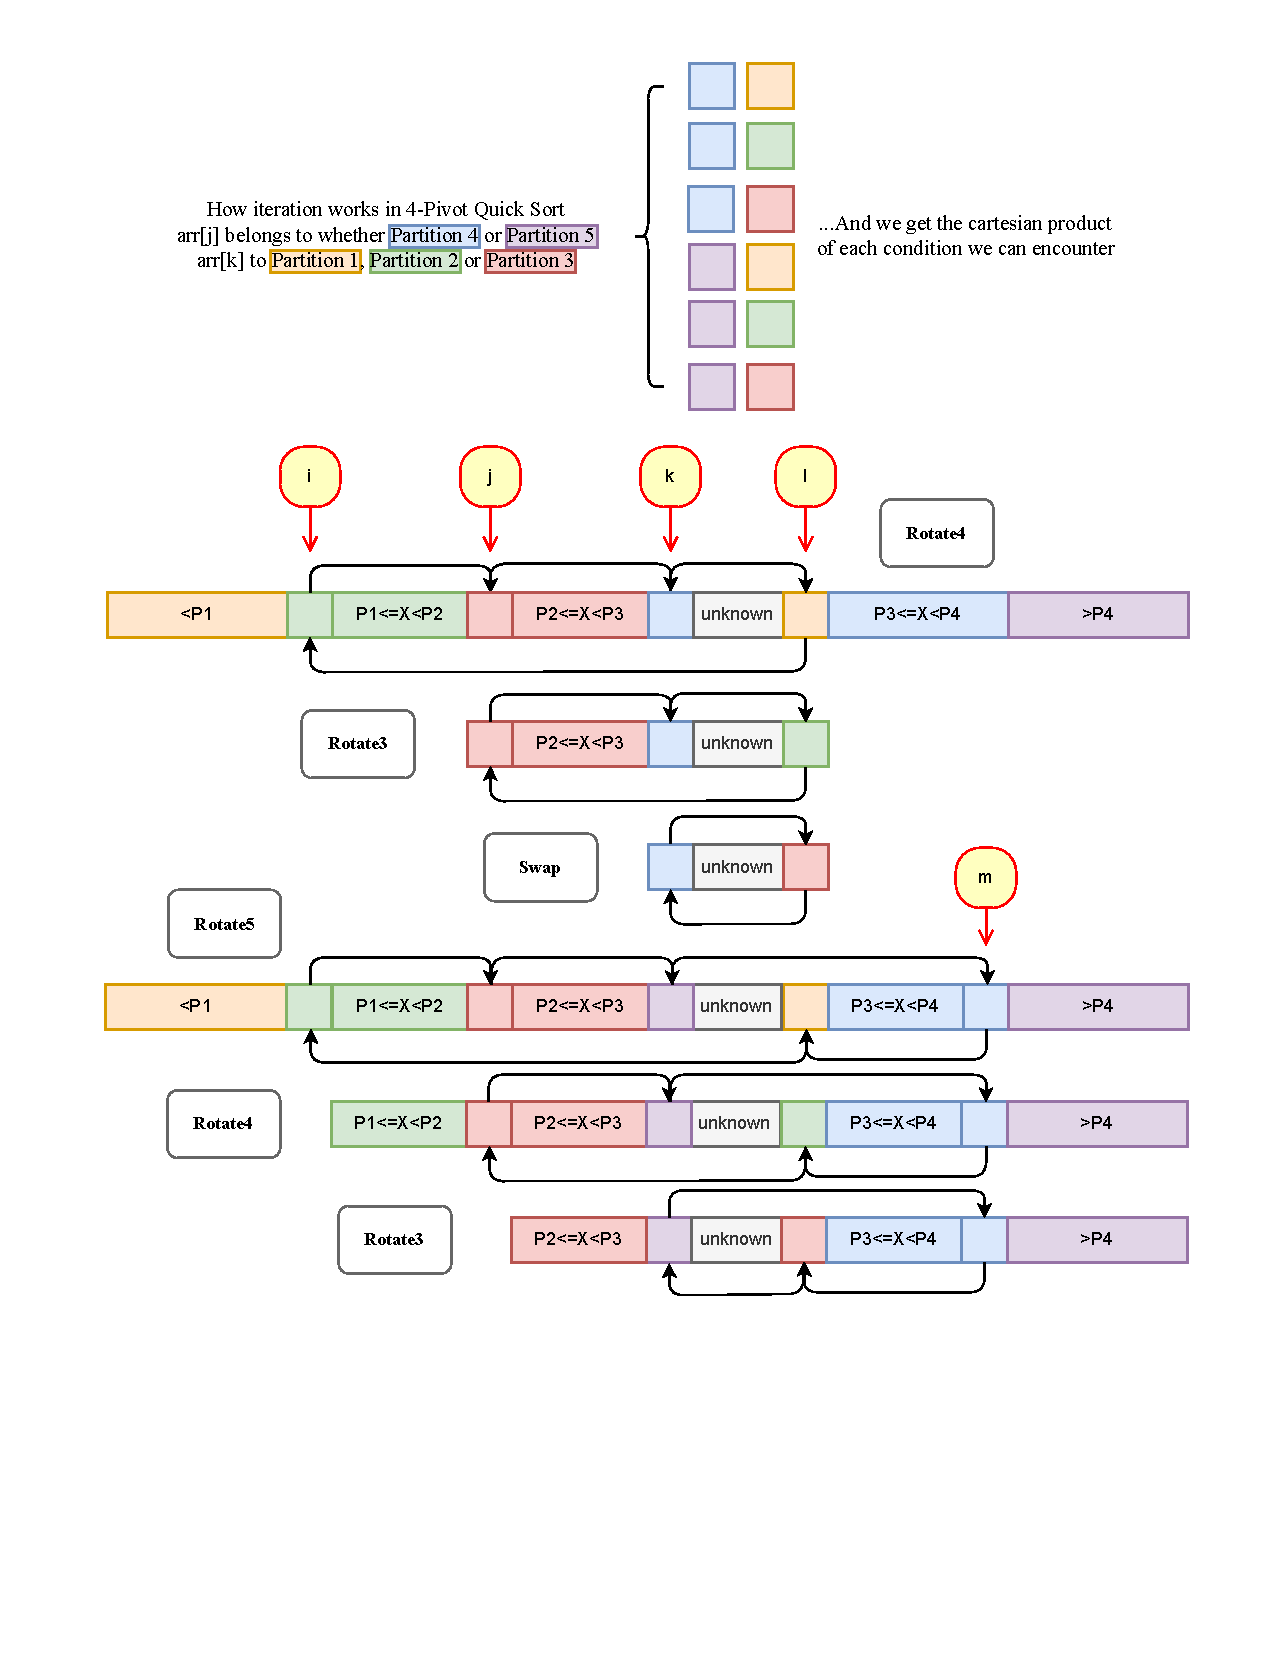
\includegraphics[width=1.5\textwidth]{4pivot.drawio.pdf}
\end{figure}


\subsection{Analysis}
The analysis on the results of Branch Misses, Cache Misses, Instructions and Time will be conducted below with regard to the Multi-Pivot QuickSorts with traditional partitions.
The details regarding to the testing machine, environment and compiler settings
\footnote{'opt-level=3' is equivalent to '-O3', 'codegen-units=1' is equivalent to '-fno-merge-all-constants', 'lto="thin"' is equivalent to '-flto=thin' in GCC.} are as follows:
\begin{center}
    \begin{tabular}{ |c|c|c|c|c| }
        \hline
        \multicolumn{2}{ | c | }{CPU}  & \multicolumn{3}{ c | }{Cache} \\
        \hline
        \multicolumn{2}{ | c | }{R7 3700x @4.3GHz Overclocked} & L1 8x32KB & L2 8x512KB & L3 2x16MB \\
        \hline
    \end{tabular}
    \begin{tabular}{ |c|c|c| }
        \hline
        RAM  & OS           & Compiler \\
        \hline
        16GB & GNU/Linux Ubuntu 22.04 & Rustc 1.78.0 +Nightly \\
        \hline
        \textbf{Rustc Flags} & \multicolumn{2}{ c | }{opt-level=3,codegen-units=1,lto="thin"} \\
        \hline
    \end{tabular}
\end{center}

All the tests above are benchmarked using the criterion library, inspired by the Haskell criterion library, which is a powerful and easy-to-use benchmarking tool for Rust.
Tests are put into groups and each group is a collection of benchmarks that are run together, with the exact same environment and the same settings.
Each test runs in a black box, which blocks the compiler from doing optimizations that are way too aggressive, such as removing instructions it thinks are redundant.
The criterion-perf-events plugin is also adapted to capture the hardware events of the CPU, with the help of the well-known profiling tool $perf$ on Linux. Why not cachegrind? Because cachegrind is a simulation tool on the cache misses and introduces a huge overhead on the runtime,
in previous tests with perf, the overall runtime appeared to have at least 200\% difference with the real-world performance, so it was rejected in the end.
Comparably, perf is a more lightweight tool that suits our needs and the given results are more reliable. Previous tests with cachegrind are given in the appendix.
% TODO: Add the appendix of cachegrind results

The compiler flags passed in are the same for all the tests, and the tests are conducted on the same machine with the same environment,
with 3 seconds of warm-up time and 5 seconds of measurement time for each test. The results are then calculated over regression tests with 100, 1000, 10000, 100000, 1000000 and 10000000 elements,
filtering out the outliers and the each item is collected with the mean, standard deviation and median. The results are shown in the tables below.
% The next part of the thesis will be the implementation of the Multi-Pivot Quicksort and the BlockQuickSort,
% followed by the analysis of the results and the comparisons on the performance of the above algorithms using traditional partition methods.
\begin{center}
    \begin{tabular}{ |c c | c c c| }
        \hline
        Branch Misses   & Size     & Mean           & SD            & Median \\
        \hline
        1-Pivot Hoare   & 100      & 224.4847       & 0.0588        & 224.4906 \\
                        & 1000     & 3612.1521      & 2.2119        & 3612.3146 \\
                        & 10000    & 49451.5958     & 72.9468       & 49464.5783 \\
                        & 100000   & 622681.4604    & 1879.7192     & 622662.0813 \\
                        & 1000000  & 7514512.0625   & 57015.6085    & 7528135.1250 \\
                        & 10000000 & 88601386.6500  & 1316610.4428  & 88910896.5000 \\
        \hline
        1-Pivot Lomuto  & 100      & 208.5500       & 0.2674        & 208.4572 \\
                        & 1000     & 3431.9977      & 4.9888        & 3432.6774 \\
                        & 10000    & 47510.1674     & 62.4065       & 47492.9219 \\
                        & 100000   & 599369.5910    & 3094.0668     & 599127.2778 \\
                        & 1000000  & 7188431.3250   & 77244.2181    & 7204133.7500 \\
                        & 10000000 & 85572728.6000  & 1273266.3095  & 85589444.5000 \\
        \hline
        2-Pivot Yaro    & 100      & 218.6639       & 0.0935        & 218.6437 \\
                        & 1000     & 3629.7245      & 1.7137        & 3630.2813 \\
                        & 10000    & 50301.2096     & 38.3586       & 50300.6213 \\
                        & 100000   & 635045.2987    & 2126.8544     & 634416.1873 \\
                        & 1000000  & 7624533.4500   & 45160.5385    & 7614424.8750 \\
                        & 10000000 & 90144952.0000  & 955908.5187   & 90243746.5000 \\
        \hline
        3-Pivot Kush    & 100      & 231.0457       & 0.0996        & 231.0266 \\
                        & 1000     & 3828.0046      & 1.7692        & 3827.5547 \\
                        & 10000    & 52692.9469     & 57.0170       & 52699.8674 \\
                        & 100000   & 660656.7803    & 2410.3154     & 660486.3048 \\
                        & 1000000  & 7881473.7500   & 55041.5020    & 7885420.7000 \\
                        & 10000000 & 93039500.9000  & 1138513.6270  & 93254088.5000 \\
        \hline
        4-Pivot         & 100      & 233.3581       & 0.1961        & 233.3429 \\
                        & 1000     & 3847.1970      & 1.7934        & 3847.1812 \\
                        & 10000    & 52466.7069     & 69.7884       & 52466.1749 \\
                        & 100000   & 655540.9742    & 2248.3174     & 655697.4468 \\
                        & 1000000  & 7831009.1900   & 49027.0168    & 7835433.7000 \\
                        & 10000000 & 92702517.3500  & 1393247.4531  & 93065712.5000 \\
        \hline
    \end{tabular}
\end{center}

The traditional means don't show much difference between the 1-Pivot Hoare and Lomuto partition methods,
it makes sense that the 1-Pivot Hoare's partition method has a slightly higher mean of branch misses than the 1-Pivot Lomuto's partition method
when Hoare's partition method seeks 2 out-of-order elements to swap, while only 1 for Lomuto's. We are bound to have some more branch misses in the former case.
But the 2-Pivot Yaro's partition method has a slightly higher mean of branch misses. The introduction of the 2nd pivot has brought more branches into concerns,
the complexities grow linearly with the number of pivots but the standard deviation grows rapidly as the size of array exceeds 10k, and explodes after 1 million.
Down follows the 3-Pivot Kush's partition method has a slightly higher mean of branch misses than the 2-Pivot Yaroslavskiy's partition method.

While things go beyond our expectations, the 4-Pivot partition shows better statistics of branch misses than the 3-Pivot partition method, which is a surprise to us,
even though it has slightly higher means of branch misses than the 2-Pivot Yaroslavskiy's partition method, the standard deviation remains at a high level indicating
the possible instabilities of the 4-Pivot partition method brought by 2 more branches \hypertarget{2MoreBranches}{`} that 1 more pivot introduced. It is still worth our notice, that it can happen when more pivots could reduce the branch misses instead of adding more burdon to the CPU.
It might be that the layout of 'balanced partition' we are using is more friendly to the CPU's branch predictor, but yet to explain why 2 more branches could bring better effects. This could be a topic in future works, further expand the research on the Multi-Pivot Quicksort algorithm. 

Apart from the branch misses, the cache misses could also play a significant factor that could affect a lot, which is what we are going to shift our focus to.

\begin{center}
    \begin{tabular}{ |c c | c c c| }
        \hline
        Cache Misses    & Size     & Mean           & SD            & Median \\
        \hline
        1-Pivot Hoare   & 100      & 0.0205         & 0.0120        & 0.0188 \\
                        & 1000     & 0.6087         & 1.4656        & 0.2268 \\
                        & 10000    & 3.4867         & 2.7533        & 2.7844 \\
                        & 100000   & 1079.6629      & 230.8850      & 996.8944 \\
                        & 1000000  & 25764.5000     & 1166.9931     & 25475.1250 \\
                        & 10000000 & 634608.9000    & 13770.3278    & 633085.5000 \\
        \hline
        1-Pivot Lomuto  & 100      & 0.0309         & 0.0585        & 0.0114 \\
                        & 1000     & 1.5477         & 2.5235        & 0.7386 \\
                        & 10000    & 16.8345        & 33.0704       & 6.4018 \\
                        & 100000   & 1033.2760      & 46.1483       & 1016.9857 \\
                        & 1000000  & 25119.6125     & 1033.3887     & 24916.1250 \\
                        & 10000000 & 653495.7500    & 17064.0432    & 653582.5000 \\
        \hline
        2-Pivot Yaro    & 100      & 0.0470         & 0.1104        & 0.0155 \\
                        & 1000     & 1.3900         & 4.3104        & 0.3234 \\
                        & 10000    & 14.0858        & 30.1847       & 6.7674 \\
                        & 100000   & 1200.8078      & 284.2979      & 1131.0076 \\
                        & 1000000  & 22058.5875     & 528.7325      & 21870.3750 \\
                        & 10000000 & 598454.2000    & 6634.4607     & 597553.5000 \\
        \hline
        3-Pivot Kush    & 100      & 0.0118         & 0.0093        & 0.0095 \\
                        & 1000     & 1.0156         & 1.9968        & 0.5050 \\
                        & 10000    & 9.3897         & 19.5556       & 4.8184 \\
                        & 100000   & 1071.0240      & 157.6619      & 1032.5982 \\
                        & 1000000  & 22472.1100     & 1444.4493     & 22098.3000 \\
                        & 10000000 & 608203.3000    & 7020.9750     & 607993.0000 \\
        \hline
        4-Pivot         & 100      & 0.0343         & 0.0814        & 0.0120 \\
                        & 1000     & 1.3838         & 2.5992        & 0.5333 \\
                        & 10000    & 4.1651         & 4.0935        & 3.1953 \\
                        & 100000   & 1158.2534      & 209.3988      & 1090.7000 \\
                        & 1000000  & 22077.3200     & 600.9565      & 22069.7000 \\
                        & 10000000 & 587479.3000    & 11805.1672    & 582773.5000 \\
        \hline
    \end{tabular}
\end{center}

The global trend shows the outburst of cache misses when scaling from 10k to 100k, possibly due to the drain of the L1 cache.
In fact, the CPU has already run out of L1 cache for size 10k, while the spatial locality of the elements is still good enough to keep the L2 cache misses at a low level.
Since L2 misses have a much larger latency than L1 misses, the performance of the algorithm is seriously affected by having to wait for the memory, this amplifies the differences between these algorithms.
Changes in rapid growth of standard deviation is also noteworthy, indicating the dramatic influences caused by the cache misses when the size of the array exceeds 10k.

In 1-Pivot tests, Lomuto shows much higher cache misses than Hoare, could be due to the fact that Lomuto's partition method has more overlapping swaps than Hoare's,
where most swaps take on the elements that are already in the right place. As the number of pivots grow, the cache misses seem to decrease, appeared in the 4-Pivot version,
might help to support the claim that 'less memory access and fewer cache misses' given the declaration above 'choosing more pivots will significantly reduce the chance we access the same elements again',
but the high level of standard deviation still remains a concern.

Among all variations the 2-Pivot Yaroslavskiy's partition method seems to have the lowest mean of both cache misses and branch misses in most of the tests, with stability in standard deviation,
it shows decent deterministic behavior, a potential good sign for the performance of the algorithm. 

For 3-Pivots, the cache behavior didn't seem to fully comply with the theoretical analysis that it is cache friendlier than classical and Yaroslavskiy's 2-Pivot QuickSorts, 
the cache misses are higher than the 2-Pivot Yaroslavskiy's partition method when the array size is larger than 1 million. The bound between cache misses and the number of pivots is not yet clear.
Contrary to the conclusion reported on experiments carried out by Kushagra's team, which supports the improvements on Multi-Pivots QuickSort are due to better cache behaviors
\cite{Kushagra}, the results of the tests conducted in this thesis show that the cache misses are not always decreasing with more pivots. For instance, the 3-Pivot Kush's has more observed cache misses than the 2-Pivot Yaroslavskiy's,
shows better performance than 2-Pivots during runtime tests. These effects are not yet fully understood and need further discussions, as I'm using Rust to implement the Multi-Pivot QuickSorts,
whose compiler is based on top of LLVM (Native LLVM as the Rust's bootstrapped backend codegen component Cranelift is far from being mature by cross-platform), that might have optimized the code in a different way that the cache behaviors are not well reflected in the results, although I enabled the most aggressive optimizations flags in the compiler settings
and they are similar as GCC and Clang's. They also reported that their 7-Pivot QuickSort has worse performance than the 3-Pivot QuickSort as a result of poor cache behaviors, which is not yet tested in this thesis.
But with the counter examples we have, we need to be more cautious about leveraging how much propotions of the performance improvements are due to better cache behaviors. It is still a topic for further research.
We will discuss about the complicated relationships further when we finish up the analysis on the instructions and time.

In the parts below, we will continue to seek more exceptions that could shift our opinions on the connections between cache and algorithm efficiency.

\begin{center}
    \begin{tabular}{ |c c | c c c| }
        \hline
        CPU Cycles      & Size     & Mean           & SD            & Median \\
        \hline
        1-Pivot Hoare   & 100      & 9327.4759      & 18.6229       & 9321.5095 \\
                        & 1000     & 141738.7953    & 210.1901      & 141718.3450 \\
                        & 10000    & 1896946.0648   & 20737.2369    & 1891616.5700 \\
                        & 100000   & 23894324.6266  & 136138.2225   & 23938976.7268 \\
                        & 1000000  & 283465722.4250 & 4456168.7125  & 282439687.8750 \\
                        & 10000000 & 3341781994.300 & 21642481.3347 & 3341179100.5000 \\
        \hline
        1-Pivot Lomuto  & 100      & 8753.9251      & 19.1779       & 8747.1730 \\
                        & 1000     & 133820.5575    & 121.5330      & 133786.0877 \\
                        & 10000    & 1797257.9908   & 1206.3404     & 1797317.9663 \\
                        & 100000   & 22592563.3050  & 184018.1868   & 22560236.2500 \\
                        & 1000000  & 266780288.5625 & 1370978.1629  & 266496379.5000 \\
                        & 10000000 & 3176006233.550 & 31963176.2929 & 3178944155.5000 \\
        \hline
        2-Pivot Yaro    & 100      & 8731.0535      & 13.1483       & 8733.6726 \\
                        & 1000     & 134846.2398    & 206.7811      & 134824.3757 \\
                        & 10000    & 1813160.2271   & 4167.9340     & 1812861.3252 \\
                        & 100000   & 22590180.7687  & 50252.7800    & 22586713.9725 \\
                        & 1000000  & 271262015.0750 & 2037510.3443  & 271168330.2500 \\
                        & 10000000 & 3222076486.750 & 22825580.2990 & 3228776030.0000 \\
        \hline
        3-Pivot Kush    & 100      & 8612.3759      & 35.5221       & 8603.2238 \\
                        & 1000     & 130997.1678    & 1591.6522     & 130493.5023 \\
                        & 10000    & 1736859.7051   & 1691.3828     & 1736487.8719 \\
                        & 100000   & 21593228.2474  & 199876.9076   & 21493032.9813 \\
                        & 1000000  & 257443837.9800 & 1733684.7359  & 256993526.2000 \\
                        & 10000000 & 3026119949.450 & 23471563.5615 & 3025067078.5000 \\
        \hline
        4-Pivot         & 100      & 8563.8790      & 9.0442        & 8562.7883 \\
                        & 1000     & 129414.4258    & 60.9929       & 129430.0027 \\
                        & 10000    & 1712788.0590   & 1490.2721     & 1712866.7067 \\
                        & 100000   & 21148019.6577  & 123063.0849   & 21104913.9275 \\
                        & 1000000  & 249836540.5700 & 1201917.2970  & 249647638.0000 \\
                        & 10000000 & 2961500698.750 & 21436898.4187 & 2957871275.5000 \\
        \hline
    \end{tabular}
\end{center}

Now it is time to deal with the total CPU cycles, the global trend is as the pivots increase, the number of CPU cycles falls.
But the 2-Pivot Yaroslavskiy's method exposed its weakness with respect to the 1-Pivot Lomuto's method. 

The 4-Pivot shows the least amount of cycles and least deviations. Combining all the factors together, the final runtime performance is reveiled as follows.

\begin{center}
    \begin{tabular}{ |c c | c c c| }
        \hline
        Time            & Size     & Mean         & SD          & Median \\
        \hline
        1-Pivot Hoare   & 100      & 2.1751 μs    & 7.3394 μs   & 2.1724 μs \\
                        & 1000     & 33.659 μs    & 203.14 μs   & 33.553 μs \\
                        & 10000    & 442.01 μs    & 2.1185 μs   & 441.58 μs \\
                        & 100000   & 5.5583 ms    & 79.072 μs   & 5.5294 ms \\
                        & 1000000  & 66.392 ms    & 1.0688 ms   & 66.594 ms \\
                        & 10000000 & 776.49 ms    & 3.7364 ms   & 776.07 ms \\
        \hline
        1-Pivot Lomuto  & 100      & 2.0334 µs    & 5.281 ns    & 2.0322 μs \\
                        & 1000     & 31.105 µs    & 123.19 ns   & 31.062 µs \\
                        & 10000    & 419.93 µs    & 3.2284 µs   & 418.01 µs \\
                        & 100000   & 5.2008 ms    & 19.270 µs   & 5.1963 ms \\
                        & 1000000  & 62.292 ms    & 452.07 µs   & 62.217 ms \\
                        & 10000000 & 745.10 ms    & 6.7564 ms   & 743.02 ms \\
        \hline
        2-Pivot Yaro    & 100      & 2.0848 µs    & 6.1677 ns   & 2.0827 µs \\
                        & 1000     & 31.372 µs    & 95.770 ns   & 31.347 µs \\
                        & 10000    & 429.91 µs    & 5.6708 µs   & 428.28 µs \\
                        & 100000   & 5.3164 ms    & 15.375 µs   & 5.3128 ms \\
                        & 1000000  & 63.092 ms    & 500.09 µs   & 62.958 ms \\
                        & 10000000 & 748.26 ms    & 4.8510 ms   & 749.60 ms \\
        \hline
        3-Pivot Kush    & 100      & 1.9985 µs    & 9.7010 ns   & 1.9943 µs \\
                        & 1000     & 30.422 µs    & 80.286 ns   & 30.392 µs \\
                        & 10000    & 411.09 µs    & 798.13 ns   & 410.84 µs \\
                        & 100000   & 5.0570 ms    & 28.975 µs   & 5.0482 ms \\
                        & 1000000  & 60.328 ms    & 906.06 µs   & 60.771 ms \\
                        & 10000000 & 717.27 ms    & 6.5670 ms   & 716.72 ms \\
        \hline
        4-Pivot         & 100      & 1.9923 µs    &	6.2348 ns   & 1.9901 µs \\
                        & 1000     & 30.422 µs    &	94.982 ns   & 30.400 µs \\
                        & 10000    & 403.15 µs    & 1.7442 µs   & 402.50 µs \\
                        & 100000   & 4.9661 ms    & 23.757 µs   & 4.9566 ms \\
                        & 1000000  & 58.758 ms    & 365.07 µs 	& 58.683 ms \\
                        & 10000000 & 696.42 ms    & 5.1556 ms   & 696.82 ms \\
        \hline
    \end{tabular}
\end{center}

% A former analysis concerning the details of the overall costs and partitioning costs has been brought by Hennequin's thesis \cite{Hennequin} in terms of Multi-Pivot QuickSorts,
% where the author proved that if the average partitioning cost for $n$ elements is $a\cdot n + O(1)$ with a constant $a$, the overall cost then will be $\frac{6}{5}a\cdot n \ln n + \bigO{n}$.
% TODO: WTF does this mean? I need to understand this first before I can write it down.

Contrary to our expectations, 2-Pivot Yaroslavskiy's method was defeated by the 1-Pivot Lomuto's method in terms of time, even though it outperformed in the cache misses.
The running time does show the correlation with the branch misses, but the cache misses don't seem to have a significant impact, where Yaroslavskiy's method has the lower cache misses but higher time than Lomuto's method.
It also has lower cache misses than Kushagra's 3-Pivot method, but the time is still much higher for larger array sizes than the 3-Pivot method.

The final running time also supports the exceptional cases above, where cache misses don't necessarily have a direct impact on the final performance of the algorithm.
The hoare partition, with 2 while loops scanning for the out-of-order elements on both sides, introduced extra overheads on branch misses and didn't manage to compete with other algorithms.
This could be the actual pain point that the 1-Pivot Hoare's method has to face, the branch misses appear to be the bottleneck, but we will soon find out the way to overcome it in the following sections.
What's enligntening is that the 4-Pivot method has the least amount of time along with less branch misses and cache misses, the improvements are made in small steps but the overall performance is promising,
although how the 4-Pivot method has more predicted branches but less actual branch misses still requires further researches.



\begin{center}
    \begin{tabular}{ |c c | c c c| }
        \hline
        Branch Misses   & Size     & Mean           & SD            & Median \\
        \hline
        1-Pivot Hoare   & 100      & 224.4847       & 0.0588        & 224.4906 \\
                        & 1000     & 3612.1521      & 2.2119        & 3612.3146 \\
                        & 10000    & 49451.5958     & 72.9468       & 49464.5783 \\
                        & 100000   & 622681.4604    & 1879.7192     & 622662.0813 \\
                        & 1000000  & 7514512.0625   & 57015.6085    & 7528135.1250 \\
                        & 10000000 & 88601386.6500  & 1316610.4428  & 88910896.5000 \\
        Block Partition & 100      & 140.5428       & 0.0876        & 140.5400 \\
                        & 1000     & 1570.7223      & 0.3938        & 1570.6199 \\
                        & 10000    & 16756.4235     & 7.9552        & 16757.5304 \\
                        & 100000   & 174650.0671    & 156.4744      & 174665.2439 \\
                        & 1000000  & 1813011.9915   & 5043.7407     & 1811789.7762 \\
                        & 10000000 & 20131908.6500  & 59866.7898    & 20134795.0000 \\
        \hline
        1-Pivot Lomuto  & 100      & 208.5500       & 0.2674        & 208.4572 \\
                        & 1000     & 3431.9977      & 4.9888        & 3432.6774 \\
                        & 10000    & 47510.1674     & 62.4065       & 47492.9219 \\
                        & 100000   & 599369.5910    & 3094.0668     & 599127.2778 \\
                        & 1000000  & 7188431.3250   & 77244.2181    & 7204133.7500 \\
                        & 10000000 & 85572728.6000  & 1273266.3095  & 85589444.5000 \\
        Block Partition & 100      & 112.3253       & 1.7694        & 112.7843 \\
                        & 1000     & 1847.2526      & 6.8858        & 1570.6199 \\
                        & 10000    & 25410.1772     & 123.7813      & 25350.7255 \\
                        & 100000   & 294244.7788    & 3465.6995     & 294878.4121 \\
                        & 1000000  & 3309146.6000   & 66124.1202    & 3313478.8000 \\
                        & 10000000 & 38173447.6500  & 1498913.4243  & 37931268.5000 \\
        \hline
        2-Pivot Yaro    & 100      & 218.6639       & 0.0935        & 218.6437 \\
                        & 1000     & 3629.7245      & 1.7137        & 3630.2813 \\
                        & 10000    & 50301.2096     & 38.3586       & 50300.6213 \\
                        & 100000   & 635045.2987    & 2126.8544     & 634416.1873 \\
                        & 1000000  & 7624533.4500   & 45160.5385    & 7614424.8750 \\
                        & 10000000 & 90144952.0000  & 955908.5187   & 90243746.5000 \\
        Lomuto Block    & 100      & 108.9624       & 0.0537        & 108.9703 \\
                        & 1000     & 1423.2516      & 3.1800        & 1422.2247 \\
                        & 10000    & 17959.2518     & 49.0859       & 17951.8464 \\
                        & 100000   & 196951.7141    & 1583.5204     & 197172.6696 \\
                        & 1000000  & 2134863.0700   & 33965.1267    & 2119311.9000 \\
                        & 10000000 & 24700025.8000  & 856684.2381   & 24551996.5000 \\
        \hline
        3-Pivot Kush    & 100      & 231.0457       & 0.0996        & 231.0266 \\
                        & 1000     & 3828.0046      & 1.7692        & 3827.5547 \\
                        & 10000    & 52692.9469     & 57.0170       & 52699.8674 \\
                        & 100000   & 660656.7803    & 2410.3154     & 660486.3048 \\
                        & 1000000  & 7881473.7500   & 55041.5020    & 7885420.7000 \\
                        & 10000000 & 93039500.9000  & 1138513.6270  & 93254088.5000 \\
        \hline
        4-Pivot         & 100      & 233.3581       & 0.1961        & 233.3429 \\
                        & 1000     & 3847.1970      & 1.7934        & 3847.1812 \\
                        & 10000    & 52466.7069     & 69.7884       & 52466.1749 \\
                        & 100000   & 655540.9742    & 2248.3174     & 655697.4468 \\
                        & 1000000  & 7831009.1900   & 49027.0168    & 7835433.7000 \\
                        & 10000000 & 92702517.3500  & 1393247.4531  & 93065712.5000 \\
        \hline
    \end{tabular}
\end{center}

\begin{center}
    \begin{tabular}{ |c c | c c c| }
        \hline
        Cache Misses    & Size     & Mean           & SD            & Median \\
        \hline
        1-Pivot Hoare   & 100      & 0.0205         & 0.0120        & 0.0188 \\
                        & 1000     & 0.6087         & 1.4656        & 0.2268 \\
                        & 10000    & 3.4867         & 2.7533        & 2.7844 \\
                        & 100000   & 1079.6629      & 230.8850      & 996.8944 \\
                        & 1000000  & 25764.5000     & 1166.9931     & 25475.1250 \\
                        & 10000000 & 634608.9000    & 13770.3278    & 633085.5000 \\
        Block Partition & 100      & 0.0308         & 0.0710        & 0.0115 \\
                        & 1000     & 0.6074         & 1.3152        & 0.1710 \\
                        & 10000    & 2.1814         & 1.5526        & 1.6280 \\
                        & 100000   & 962.7563       & 36.5304       & 957.6906 \\
                        & 1000000  & 22939.3449     & 772.0659      & 22956.2750 \\
                        & 10000000 & 618067.7500    & 15870.0637    & 615660.5000 \\
        \hline
        1-Pivot Lomuto  & 100      & 0.0309         & 0.0585        & 0.0114 \\
                        & 1000     & 1.5477         & 2.5235        & 0.7386 \\
                        & 10000    & 16.8345        & 33.0704       & 6.4018 \\
                        & 100000   & 1033.2760      & 46.1483       & 1016.9857 \\
                        & 1000000  & 25119.6125     & 1033.3887     & 24916.1250 \\
                        & 10000000 & 653495.7500    & 17064.0432    & 653582.5000 \\
        Block Partition & 100      & 0.0382         & 0.0290        & 0.0314 \\
                        & 1000     & 0.3182         & 0.2477        & 0.2104 \\
                        & 10000    & 3.3952         & 3.7817        & 2.3033 \\
                        & 100000   & 1170.8087      & 38.3259       & 1170.6985 \\
                        & 1000000  & 25346.0800     & 820.9205      & 25164.7000 \\
                        & 10000000 & 664360.6000    & 21405.0063    & 659137.5000 \\
        \hline
        2-Pivot Yaro    & 100      & 0.0470         & 0.1104        & 0.0155 \\
                        & 1000     & 1.3900         & 4.3104        & 0.3234 \\
                        & 10000    & 14.0858        & 30.1847       & 6.7674 \\
                        & 100000   & 1200.8078      & 284.2979      & 1131.0076 \\
                        & 1000000  & 22058.5875     & 528.7325      & 21870.3750 \\
                        & 10000000 & 598454.2000    & 6634.4607     & 597553.5000 \\
        Lomuto Block    & 100      & 0.0882         & 0.2168        & 0.0370 \\
                        & 1000     & 1.6396         & 5.9674        & 0.2243 \\
                        & 10000    & 5.6262         & 2.8924        & 5.2277 \\
                        & 100000   & 1160.9140      & 51.9771       & 1143.0456 \\
                        & 1000000  & 24010.0300     & 790.7382      & 24020.7000 \\
                        & 10000000 & 635062.3500    & 14272.0662    & 634228.5000 \\
        \hline
        3-Pivot Kush    & 100      & 0.0118         & 0.0093        & 0.0095 \\
                        & 1000     & 1.0156         & 1.9968        & 0.5050 \\
                        & 10000    & 9.3897         & 19.5556       & 4.8184 \\
                        & 100000   & 1071.0240      & 157.6619      & 1032.5982 \\
                        & 1000000  & 22472.1100     & 1444.4493     & 22098.3000 \\
                        & 10000000 & 608203.3000    & 7020.9750     & 607993.0000 \\
        \hline
        4-Pivot         & 100      & 0.0343         & 0.0814        & 0.0120 \\
                        & 1000     & 1.3838         & 2.5992        & 0.5333 \\
                        & 10000    & 4.1651         & 4.0935        & 3.1953 \\
                        & 100000   & 1158.2534      & 209.3988      & 1090.7000 \\
                        & 1000000  & 22077.3200     & 600.9565      & 22069.7000 \\
                        & 10000000 & 587479.3000    & 11805.1672    & 582773.5000 \\
        \hline
    \end{tabular}
\end{center}

\begin{center}
    \begin{tabular}{ |c c | c c c| }
        \hline
        CPU Cycles      & Size     & Mean           & SD            & Median \\
        \hline
        1-Pivot Hoare   & 100      & 9327.4759      & 18.6229       & 9321.5095 \\
                        & 1000     & 141738.7953    & 210.1901      & 141718.3450 \\
                        & 10000    & 1896946.0648   & 20737.2369    & 1891616.5700 \\
                        & 100000   & 23894324.6266  & 136138.2225   & 23938976.7268 \\
                        & 1000000  & 283465722.4250 & 4456168.7125  & 282439687.8750 \\
                        & 10000000 & 3341781994.300 & 21642481.3347 & 3341179100.5000 \\
        Block Partition & 100      & 7261.6214      & 3.9023        & 7261.0766 \\
                        & 1000     & 91497.6734     & 44.2229       & 91503.7709 \\
                        & 10000    & 1093098.0648   & 28276.9430    & 1087067.0555 \\
                        & 100000   & 12615251.1810  & 408397.6682   & 12525100.7167 \\
                        & 1000000  & 142142979.8257 & 1816742.9514  & 141750443.9091 \\
                        & 10000000 & 1651547110.850 & 15522352.0233 & 1651945749.0000 \\
        \hline
        1-Pivot Lomuto  & 100      & 8753.9251      & 19.1779       & 8747.1730 \\
                        & 1000     & 133820.5575    & 121.5330      & 133786.0877 \\
                        & 10000    & 1797257.9908   & 1206.3404     & 1797317.9663 \\
                        & 100000   & 22592563.3050  & 184018.1868   & 22560236.2500 \\
                        & 1000000  & 266780288.5625 & 1370978.1629  & 266496379.5000 \\
                        & 10000000 & 3176006233.550 & 31963176.2929 & 3178944155.5000 \\
        Block Partition & 100      & 7008.9387      & 28.2391       & 7005.8331 \\
                        & 1000     & 119936.7616    & 332.2665      & 120045.5206 \\
                        & 10000    & 1635196.2005   & 3174.6739     & 1635068.8220 \\
                        & 100000   & 19944485.2959  & 165665.3166   & 19999479.0516 \\
                        & 1000000  & 234756806.7100 & 3512955.3454  & 233878365.1000 \\
                        & 10000000 & 2779056745.450 & 88165361.1430 & 2783135055.5000 \\
        \hline
        2-Pivot Yaro    & 100      & 8731.0535      & 13.1483       & 8733.6726 \\
                        & 1000     & 134846.2398    & 206.7811      & 134824.3757 \\
                        & 10000    & 1813160.2271   & 4167.9340     & 1812861.3252 \\
                        & 100000   & 22590180.7687  & 50252.7800    & 22586713.9725 \\
                        & 1000000  & 271262015.0750 & 2037510.3443  & 271168330.2500 \\
                        & 10000000 & 3222076486.750 & 22825580.2990 & 3228776030.0000 \\
        Lomuto Block    & 100      & 6921.2645      & 7.4863        & 6920.0053 \\
                        & 1000     & 115531.6098    & 1531.6089     & 115046.6171 \\
                        & 10000    & 1567567.6369   & 5508.4648     & 1567416.7897 \\
                        & 100000   & 18897769.3384  & 175912.1206   & 18848614.8083 \\
                        & 1000000  & 216844641.5500 & 2817917.2648  & 216536644.3000 \\
                        & 10000000 & 2548418986.850 & 48249924.4893 & 2559985148.0000 \\
        \hline
        3-Pivot Kush    & 100      & 8612.3759      & 35.5221       & 8603.2238 \\
                        & 1000     & 130997.1678    & 1591.6522     & 130493.5023 \\
                        & 10000    & 1736859.7051   & 1691.3828     & 1736487.8719 \\
                        & 100000   & 21593228.2474  & 199876.9076   & 21493032.9813 \\
                        & 1000000  & 257443837.9800 & 1733684.7359  & 256993526.2000 \\
                        & 10000000 & 3026119949.450 & 23471563.5615 & 3025067078.5000 \\
        \hline
        4-Pivot         & 100      & 8563.8790      & 9.0442        & 8562.7883 \\
                        & 1000     & 129414.4258    & 60.9929       & 129430.0027 \\
                        & 10000    & 1712788.0590   & 1490.2721     & 1712866.7067 \\
                        & 100000   & 21148019.6577  & 123063.0849   & 21104913.9275 \\
                        & 1000000  & 249836540.5700 & 1201917.2970  & 249647638.0000 \\
                        & 10000000 & 2961500698.750 & 21436898.4187 & 2957871275.5000 \\
        \hline
    \end{tabular}
\end{center}
\begin{center}
    \begin{tabular}{ |c c | c c c| }
        \hline
        Time            & Size     & Mean         & SD          & Median \\
        \hline
        1-Pivot Hoare   & 100      & 2.1751 μs    & 7.3394 μs   & 2.1724 μs \\
                        & 1000     & 33.659 μs    & 203.14 μs   & 33.553 μs \\
                        & 10000    & 442.01 μs    & 2.1185 μs   & 441.58 μs \\
                        & 100000   & 5.5583 ms    & 79.072 μs   & 5.5294 ms \\
                        & 1000000  & 66.392 ms    & 1.0688 ms   & 66.594 ms \\
                        & 10000000 & 776.49 ms    & 3.7364 ms   & 776.07 ms \\
        Block Partition & 100      & 1.6938 µs    & 4.7546 ns   & 1.6926 µs \\
                        & 1000     & 21.782 µs    & 107.85 ns   & 21.743 µs \\
                        & 10000    & 259.09 µs    & 490.99 ns   & 258.97 µs \\
                        & 100000   & 2.9872 ms    & 9.5993 µs   & 2.9855 ms \\
                        & 1000000  & 33.808 ms 	  & 159.14 µs   & 33.788 ms \\
                        & 10000000 & 394.79 ms    & 2.9162 ms   & 395.56 ms \\
        \hline
        1-Pivot Lomuto  & 100      & 2.0334 µs    & 5.281 ns    & 2.0322 μs \\
                        & 1000     & 31.105 µs    & 123.19 ns   & 31.062 µs \\
                        & 10000    & 419.93 µs    & 3.2284 µs   & 418.01 µs \\
                        & 100000   & 5.2008 ms    & 19.270 µs   & 5.1963 ms \\
                        & 1000000  & 62.292 ms    & 452.07 µs   & 62.217 ms \\
                        & 10000000 & 745.10 ms    & 6.7564 ms   & 743.02 ms \\
        Block Partition & 100      & 1.6698 µs    & 4.2852 ns   & 1.6689 µs \\
                        & 1000     & 28.453 µs    & 87.002 ns   & 28.424 µs \\
                        & 10000    & 392.02 µs    & 1.3621 µs   & 391.81 µs \\
                        & 100000   & 4.7857 ms    & 42.338 µs   & 4.7824 ms \\
                        & 1000000  & 56.288 ms    & 884.73 µs   & 56.358 ms \\
                        & 10000000 & 668.14 ms    & 21.283 ms   & 662.61 ms \\
        \hline
        2-Pivot Yaro    & 100      & 2.0848 µs    & 6.1677 ns   & 2.0827 µs \\
                        & 1000     & 31.372 µs    & 95.770 ns   & 31.347 µs \\
                        & 10000    & 429.91 µs    & 5.6708 µs   & 428.28 µs \\
                        & 100000   & 5.3164 ms    & 15.375 µs   & 5.3128 ms \\
                        & 1000000  & 63.092 ms    & 500.09 µs   & 62.958 ms \\
                        & 10000000 & 748.26 ms    & 4.8510 ms   & 749.60 ms \\
        Lomuto Block    & 100      & 1.6387 µs    & 4.3470 ns   & 1.6373 µs \\
                        & 1000     & 27.249 µs    & 52.407 ns   & 27.249 µs \\
                        & 10000    & 374.62 µs    & 3.3842 µs   & 373.88 µs \\
                        & 100000   & 4.5048 ms    & 31.057 µs   & 4.5022 ms \\
                        & 1000000  & 52.149 ms    & 802.78 µs   & 52.234 ms \\
                        & 10000000 & 605.61 ms    & 13.676 ms   & 602.31 ms \\
        \hline
        3-Pivot Kush    & 100      & 1.9985 µs    & 9.7010 ns   & 1.9943 µs \\
                        & 1000     & 30.422 µs    & 80.286 ns   & 30.392 µs \\
                        & 10000    & 411.09 µs    & 798.13 ns   & 410.84 µs \\
                        & 100000   & 5.0570 ms    & 28.975 µs   & 5.0482 ms \\
                        & 1000000  & 60.328 ms    & 906.06 µs   & 60.771 ms \\
                        & 10000000 & 717.27 ms    & 6.5670 ms   & 716.72 ms \\
        \hline
        4-Pivot         & 100      & 1.9923 µs    &	6.2348 ns   & 1.9901 µs \\
                        & 1000     & 30.422 µs    &	94.982 ns   & 30.400 µs \\
                        & 10000    & 403.15 µs    & 1.7442 µs   & 402.50 µs \\
                        & 100000   & 4.9661 ms    & 23.757 µs   & 4.9566 ms \\
                        & 1000000  & 58.758 ms    & 365.07 µs 	& 58.683 ms \\
                        & 10000000 & 696.42 ms    & 5.1556 ms   & 696.82 ms \\
        \hline
    \end{tabular}
\end{center}



\begin{thebibliography}{99}

\bibitem{HoareQuickSort} \label{HoareQuickSort} Hoare, C.A.R. (1962). Quicksort. \textit{The Computer Journal}, 5, 10-15.
\bibitem{Yaroslavskiy} \label{Yaroslavskiy} Yaroslavskiy, V. (2009). Dual-Pivot Quicksort. \textit{Proceedings of the 6th International Conference on Computer Science and Education}, 13-27.
\bibitem{Sedgewick} \label{Sedgewick} Sedgewick, R. (1978). Implementing Quicksort Programs. \textit{Communications of the ACM}, 21(10), 847-857.
\bibitem{Kushagra} \label{Kushagra} {Shrinu Kushagra, Alejandro López-Ortiz, Aurick Qiao, and J. Ian Munro. \textit{Multi-pivot quicksort: Theory and experiments.} In ALENEX, pages 47-60, 2014.}
\bibitem{Introsort} \label{Introsort} David R. Musser. \textit{Introspective Sorting and Selection Algorithms.} Software: Practice and Experience, 27(8):983-993, 1997.
\bibitem{BlockQuickSort} \label{BlockQuickSort} BlockQuicksort: How Branch Mispredictions don't affect Quicksort. \textit{Stefan Edelkamp and Armin Weiß.} 2016.
\bibitem{OptimalPartitioningForDualPivotQuicksort} \label{OptimalPartitioningForDualPivotQuicksort} Martin Aumüller and Martin Dietzfelbinger. 2013. \textit{Optimal Partitioning for Dual Pivot Quicksort}. In Proc.
of the 40th International Colloquium on Automata, Languages and Programming (ICALP'13). Springer, 33-44.
\bibitem{Hennequin} \label{Hennequin} Hennequin, P. (1991) \textit{Analyse en moyenne d'algorithmes: Tri rapide et arbres de recherche.} Ph.D. Thesis, Ecole Politechnique, Palaiseau.
\end{thebibliography}

\end{document}